\chapter{計算機数学}\label{chapt_computer}

{\small 「近道を探したらいけん。その先は行き止まりだ」...
NHKの連ドラ「ゲゲゲの女房」より。\hv}

\section{計算機数学}



計算機は指示されたことを極めて忠実・正確に実行する。
だから, 適切に指示されれば非常に有能だし, そうでなければ全く無能
である。だから, 計算機を使う仕事は, やり方(計算機への指示の仕方)
によって, 残酷なくらい効率に大きな差が生じる。うまくやれば5分間
で終わる仕事が, まずくやると1週間かかっても終わらないという
ことがよくある。とにかくたくさん試してたくさん失敗し, 工夫を覚えていく
しかない。そこで覚えてほしい古典的な格言がいくつかある:\\

「ひとつのことをするにもいろんな方法がある」... 計算機には様々な機能
があり, 互いに重複していることが多い。少しの知識しかない初心者でも, その知識の
中で工夫すれば, 結構いろんなことができるのだ。自分の武器で戦えば
いいのだ。\\

「楽するための苦労を厭うな」... 自分の武器で戦えばいいとは言え, 
効率的でスマートなアプローチを見出せると, やはり有利だ。そのためには, 
調べたり頭を使ったりという「苦労」が必要になる。\textgt{楽をする
ノウハウは, 苦労しないと身につかない}のだ。楽をするノウハウは, 
\textgt{上級者から盗む}のが常道である。計算機が得意な
友人の隣に座って, 友人がどのように計算機を使うのかを観察し, 
質問するのだ。\\

「困ったらググれ」 ... ネット検索は非常に強力である。
君が出会うトラブルの多くは既にネットに情報が出ている。
\textgt{解決策をネット検索で見つけ出すスキル}
が重要である。これも試行錯誤して苦労しないと身につかない。\\

「タコは育てろ」... 計算機業界では初心者を\underline{タコ} \index{たこ@タコ}
という。最初は誰でもタコである。上級者は, めんどくさくても, 
タコの\textgt{面倒をみてやる}のだ。タコが育てば, いつかは立場
が逆転して, 自分を教えてくれるようになる。\\

なお, 以下の課題のレポートを作成するときは, 両面印刷でも
構わない。\\







\section{媒介変数表示された関数のグラフ}
実数$\theta$がいろんな値をとるときに, 点$(x,y)=(\cos \theta, \sin \theta)$は, $xy$平面上で原点を中心とする
半径1の円を描く(三角関数の定義から明らか)。このように, ある共通の変数(この場合は$\theta$)
の関数として$x$と$y$のそれぞれを与えることで, 
関数のグラフ(特に陰関数のグラフ)を描くことができる。そのような変数を\underline{媒介変数}
\index{ばいかいへんすう@媒介変数}または「パラメータ」\index{ぱらめーた@パラメータ}
と呼ぶ\footnote{この「パラメータ」は, 第\ref{chapt_function}章で出てきた「パラメータ」とは意味が違うことに注意。}。
媒介変数で表現される関数のグラフは, 表計算ソフトで簡単に描くことができる。

\begin{exmpl} 円のグラフ(単位円)を描いてみよう。まず, 下記のようなスプレッドシートを用意する:\\
\begin{tabular}{|>{\columncolor[gray]{0.8}}c|c|c|c|} \hline
\rowcolor[gray]{0.8}  & A & B & C \\ \hline
1 & theta & cos & sin \\ \hline
2 & 0   &      &  \\ \hline
3 &     &      &  \\ \hline
$\vdots$ & $\vdots$ & $\vdots$ & $\vdots$ \\ \hline
\end{tabular}\\
例によって, 第1行(A1, B1, C1)は, 単なるメモである。

第A列(A2, A3, A4, ...)には, 媒介変数$\theta$の値が入る。0から出発して$2\pi$まで, 0.1きざみで入れてみよう。
そのために, セルA3には, 「=A2+0.1」と入れて, セルA4からセルA65くらいまでペーストする。また, 第B列と第C列
にはそれぞれ$x=\cos \theta$と$y=\sin \theta$が入るので, セルB2に「=cos(A2)」, セルC2に「=sin(A2)」
と入れて, それらを第65行くらいまでコピーペーストする。次のようになっただろうか?:\\
\begin{tabular}{|>{\columncolor[gray]{0.8}}c|c|c|c|} \hline
\rowcolor[gray]{0.8}  & A & B & C \\ \hline
1 & theta & cos & sin \\ \hline
2 & 0   &     1&     0\\ \hline
3 & 0.1 &     1&   0.1\\ \hline
4 & 0.2 &  0.98&   0.2\\ \hline
5 & 0.3 &  0.96&   0.3\\ \hline
$\vdots$ & $\vdots$ & $\vdots$& $\vdots$\\ \hline
65 & 6.3 &  1&   0.02\\ \hline
\end{tabular}\\

あとは, 第B列と第C列 (\underline{B2から}C65まで)を選択してグラフ(散布図\index{さんぷず@散布図})
を描けば, 円が現れるだろう。(例おわり)\\\end{exmpl}

\begin{freqmiss}{\small\textgt{上の例で, 間違って第A列と第B列を選択してグラフを描いてしまう} ... 
その場合は, 円にはならないで, $y=\cos x$のグラフになってしまう。\\}\end{freqmiss}

\begin{faq}{\small\textgt{今回はなぜB2から選んだのですか? 例\ref{exmpl:graph_y=x^2}では
A1からでしたよね?} ... まず, 第A列から選んでしまうと, 第A列が$x$軸になってしまうので, 
$y=\cos x$と$y=\sin x$のグラフになってしまい, 円にはなりません。次に, B1から選んで
しまうと, C1のメモ"sin"が凡例に表示されてしまいます。このグラフはsinのグラフではなく
円のグラフなので, sinという凡例は頂けない。そこで, あえて凡例を表示させないために, 
B2から選んだのです。\\}\end{faq}

\begin{q}\label{q:comp_graph1} 以下, $\theta$を媒介変数とし, $(x, y)$が以下のように定義された関数のグラフをパソコンで描け。ただし, 
$-\pi \le \theta \le \pi$とする。$\pi$の値は3.1415とせよ。
\begin{enumerate}
\item $(\cos \theta,\, \sin \theta)$
\item $(\cos \theta,\, \sin (\theta+\pi/3))$
\item $(\cos 3\theta,\,  \sin 4\theta)$\\(このような図形をリサジュー図形\index{りさじゅーずけい@リサジュー図形}という)
\item $((0.5\cos 5\theta+1) \cos \theta,\, (0.5\cos 5\theta+1) \sin \theta)$
\end{enumerate}\end{q}

\begin{faq}{\small\textgt{$\pi$の値は, 3.1415なんて入れなくても, 
PI()と打てばいいのに} ... よく知っていますね。このソフトでは円周率をPI()で表せます。
だから, =sin(A2+PI()/3)のように打っても, うまくいきますね。5桁以上の正確な計算が
必要なときはその方が良いでしょう。上記のようにわざわざ値で入れるのは, 前述
した可搬性のため, そして, シンプルに教えるための教育的配慮です。\\}\end{faq}

\begin{faq}{\small\textgt{問\ref{q:comp_graph1}の(1)がどうやっても
円になりません} ... もう一度, 上の解説をしっかり読むこと。$\theta$の列(第A列)と
$\cos\theta$の列(第B列)と$\sin\theta$の列(第C列)を作ったら, 
\textgt{$\theta$の列(第A列)は選ばないで}, 
$\cos\theta$の列(第B列)と$\sin\theta$の列(第C列)だけを選んで, グラフのメニューから
\textgt{散布図を選ぶ}。それでもダメなら質問においで!}\end{faq}
\vv



\section*{演習問題}

\begin{exq}\label{q:clothoid} クロソイド曲線というものをネット等で調べ, 
それを表計算ソフトで描け。この課題には, 本章で学んだこと全てが詰まっている!\end{exq}

\vv


\section*{問題の解答}


% 以下, $t, \theta$を媒介変数とし, $(x, y)$が以下のように定義された関数のグラフを
\noindent{\textbf{答}}\ref{q:comp_graph1}  図\ref{fig:cmp_circle}, 図\ref{fig:cmp_ellipse1}, 
       図\ref{fig:cmp_Lissajous}, 図\ref{fig:cmp_Hitode}
\begin{figure}[!h]
    \centering
    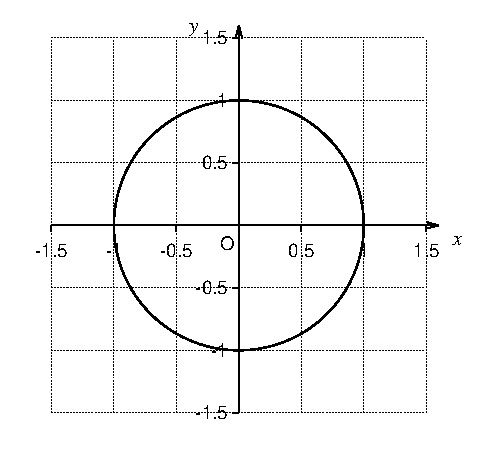
\includegraphics[width=7.0cm]{cmp_circle.eps}
    \caption{$(\cos \theta,\, \sin \theta)$のグラフ。\label{fig:cmp_circle}}
\end{figure}

\begin{figure}[!h]
    \centering
    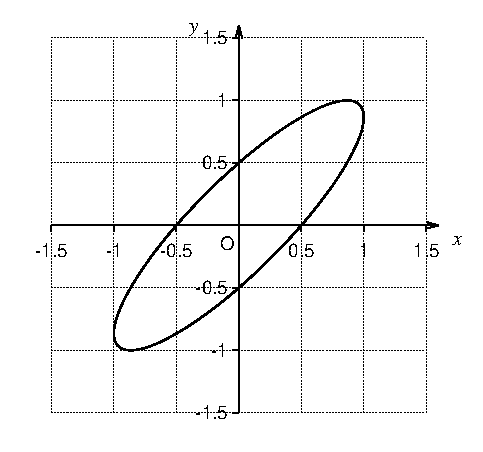
\includegraphics[width=7.0cm]{cmp_ellipse1.eps}
    \caption{$(\cos \theta,\, \sin (\theta+\pi/3))$のグラフ。\label{fig:cmp_ellipse1}}
\end{figure}

\begin{figure}[!h]
    \centering
    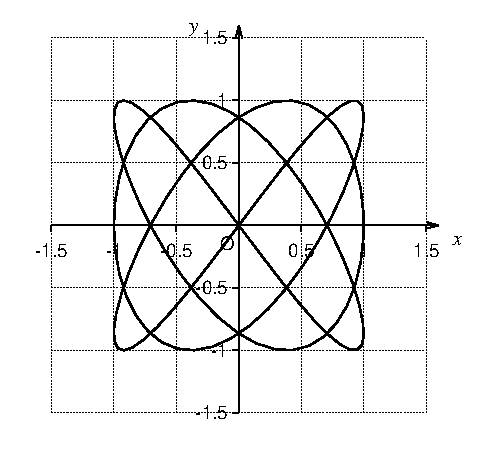
\includegraphics[width=7.0cm]{cmp_Lissajous.eps}
    \caption{$(\cos 3\theta,\,  \sin 4\theta)$のグラフ。\label{fig:cmp_Lissajous}}
\end{figure}

\begin{figure}[!h]
    \centering
    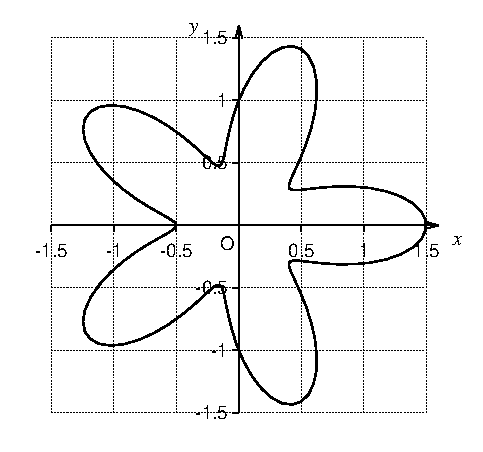
\includegraphics[width=7.0cm]{cmp_Hitode.eps}
    \caption{$((0.5\cos 5\theta+1) \cos \theta,\, (0.5\cos 5\theta+1) \sin \theta)$のグラフ。\label{fig:cmp_Hitode}}
\end{figure}


% \section{数値微分}

% 表計算ソフトで, 関数$f(x)=\exp x$を, $-2 \le x \le 2$の範囲で数値微分し, 
\noindent{\textbf{答}}\ref{q:comp_diff2}  図\ref{fig:graph_expxdiff}
\begin{figure}[!h]
    \centering
    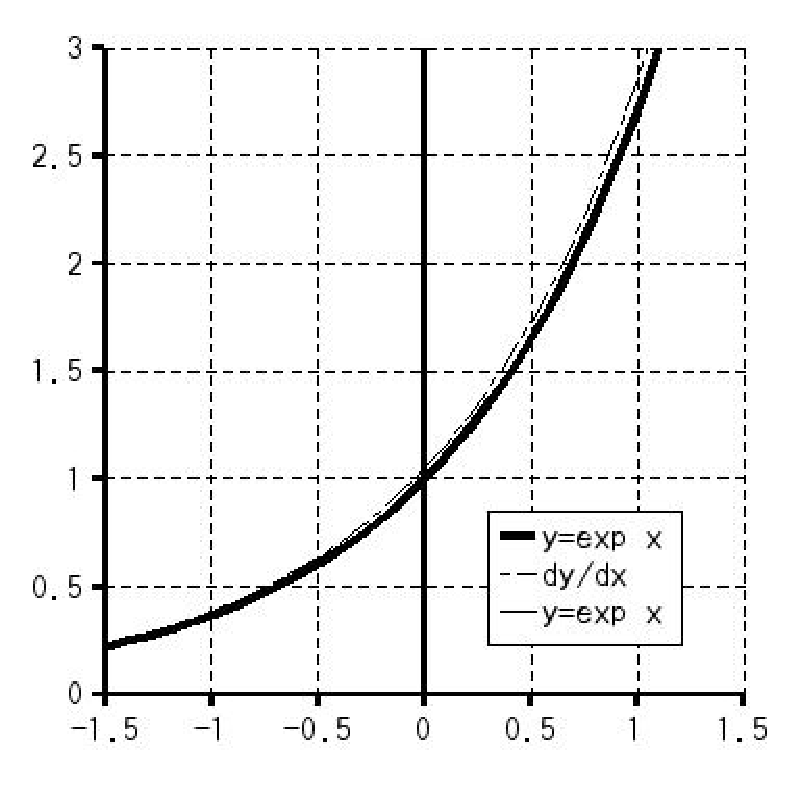
\includegraphics[width=7.5cm]{graph_expxdiff.eps}
    \caption{$y=e^x$とその数値微分(dy/dx)。\label{fig:graph_expxdiff}}
\end{figure}

% 表計算ソフトで, 関数$f(x)=\cos x$を, $0 \le x \le 7$の範囲で数値微分し, 
\noindent{\textbf{答}}\ref{q:comp_diff4}  図\ref{fig:graph_cosxdiff}
\begin{figure}[!h]
    \centering
    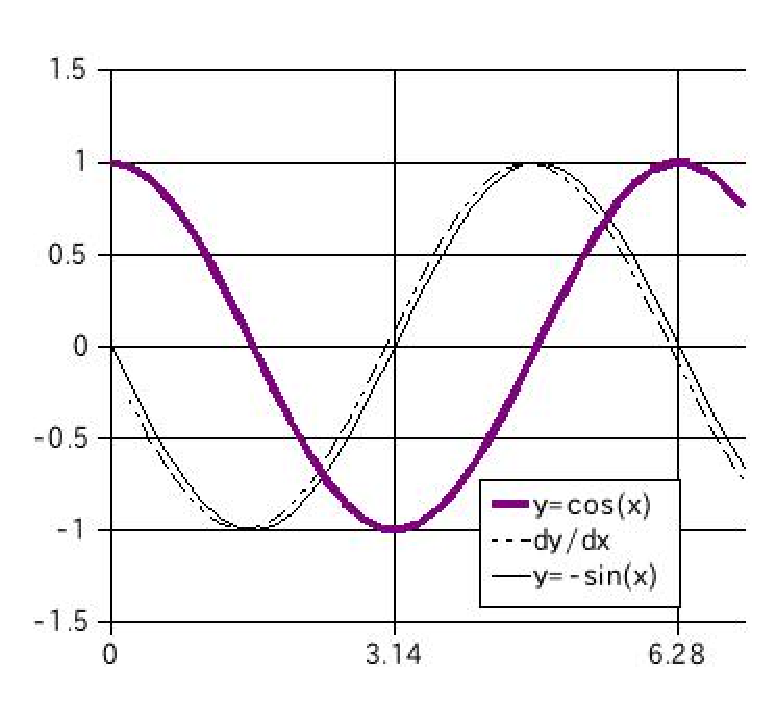
\includegraphics[width=7.0cm]{graph_cosxdiff.eps}
    \caption{$y=\cos x$とその数値微分(dy/dx)。\label{fig:graph_cosxdiff}}
\end{figure}


% \section{数値積分}

% 表計算ソフトで, 関数$f(x)=x$を, $0 \le x \le 2$の範囲で数値積分し,
\noindent{\textbf{答}}\ref{q:comp_int0}  図\ref{fig:graph_xinteg}
\begin{figure}[!h]
    \centering
    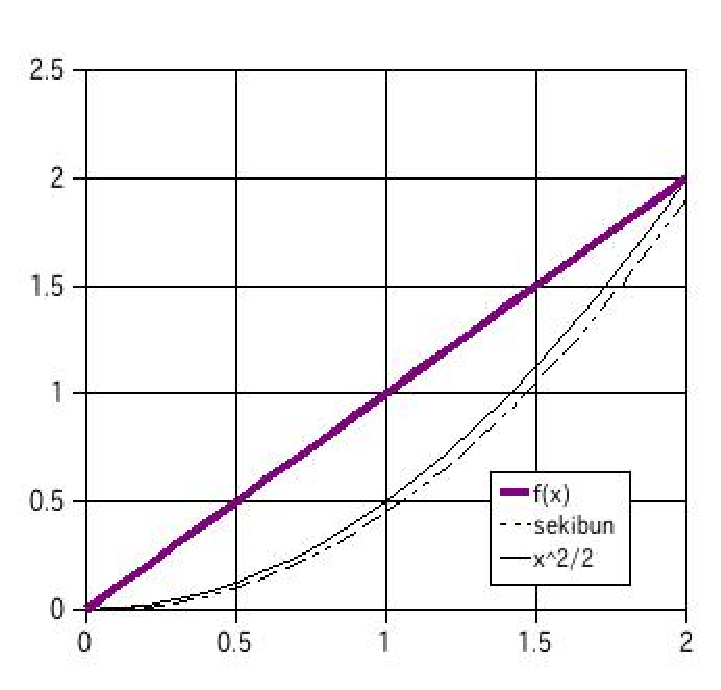
\includegraphics[width=7.0cm]{graph_xinteg.eps}
    \caption{$y=x$とその数値積分。\label{fig:graph_xinteg}}
\end{figure}

% 表計算ソフトで, 関数$f(x)=\cos x$を, $0 \le x \le 7$の範囲で数値積分し, 
\noindent{\textbf{答}}\ref{q:comp_int2}  図\ref{fig:graph_cosxinteg}
\begin{figure}[!h]
    \centering
    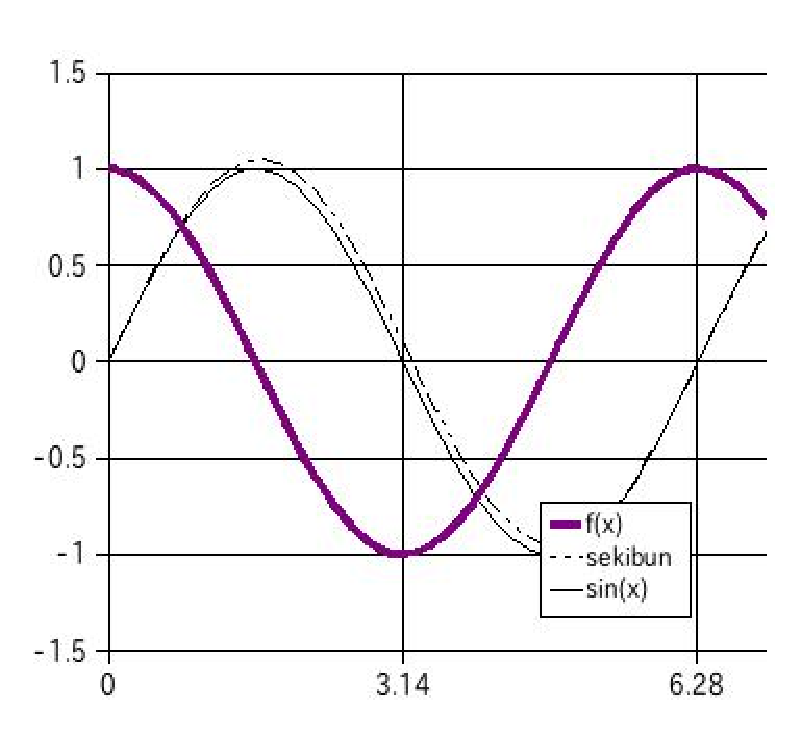
\includegraphics[width=7.0cm]{graph_cosxinteg.eps}
    \caption{$y=\cos x$とその数値積分。\label{fig:graph_cosxinteg}}
\end{figure}

% 表計算ソフトで, ガウス関数$f(x)=\exp (-x^2)$を, $-4 \le x \le 4$の範囲で数値積分し,
\noindent{\textbf{答}}\ref{q:comp_int4}  図\ref{fig:PC_graph_Gauss_integ}
\begin{figure}[!h]
    \centering
    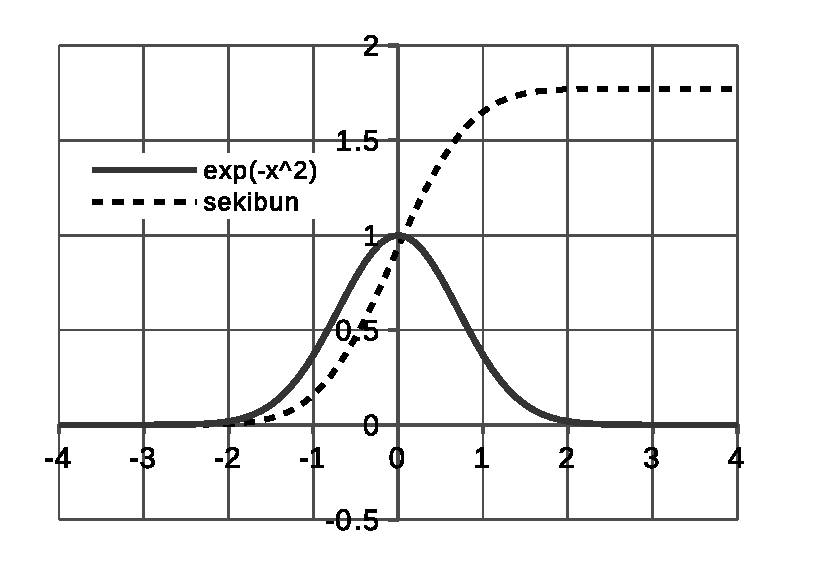
\includegraphics[width=7.5cm]{PC_graph_Gauss_integ.eps}
    \caption{$y=\exp(-x^2)$とその数値積分。\label{fig:PC_graph_Gauss_integ}}
\end{figure}
\vv



